%! Author = taj
%! Date = 7/22/25

% Preamble
\documentclass[11pt]{article}

% Packages
\usepackage{amsmath}
\usepackage{graphicx}
\usepackage{float}
\usepackage{upgreek}

\title{1. Merjenje moči mšic in nog}
\author{Taj Šobot}

% Document
\begin{document}
    \maketitle
    \flushleft
    Pri tem eksperimentu smo preučevali kako je koeficient vzmeti odvisen od njenih geometrijskih lastnosti.

    \section{Meritve}
    Merili smo 7 različnih vzmeti.
    Vsakosmo obremenili za 3 stopnje.
    Meritve teh so sledeče:
    \\
    Vzmet 1:
    \begin{table}[H]
        \centering
        \begin{tabular}{|r|r|}
            \hline
            \textbf{F} & \textbf{x} \\
            \hline
            0 & 0 \\
            19.56114 & 0.115 \\
            8.30907 & 0.034 \\
            \hline
        \end{tabular}
        \caption{}
        \label{tab:1}
    \end{table}
    Vzmet 2:
    \begin{table}[H]
        \centering
        \begin{tabular}{|r|r|}
            \hline
            \textbf{F} & \textbf{x} \\
            \hline
            0 & 0 \\
            19.56114 & 0.044 \\
            23.84811 & 0.055 \\
            \hline
        \end{tabular}
        \caption{}
        \label{tab:2}
    \end{table}
    Vzmet 3:
    \begin{table}[H]
        \centering
        \begin{tabular}{|r|r|}
            \hline
            \textbf{F} & \textbf{x} \\
            \hline
            0 & 0 \\
            19.56114 & 0.144 \\
            8.30907 & 0.048 \\
            \hline
        \end{tabular}
        \caption{}
        \label{tab:3}
    \end{table}
    Vzmet 4:
    \begin{table}[H]
    \centering
    \begin{tabular}{|r|r|}
        \hline
        \textbf{F} & \textbf{x} \\
        \hline
        0 & 0 \\
        19.56114 & 0.158 \\
        8.30907 & 0.055 \\
        \hline
    \end{tabular}
    \caption{}
    \label{tab:4}
    \end{table}
    Vzmet 5:

    \begin{table}[H]
        \centering
        \begin{tabular}{|r|r|}
            \hline
            \textbf{F} & \textbf{x} \\
            \hline
            0 & 0 \\
            19.56114 & 0.183 \\
            8.30907 & 0.068 \\
            \hline
        \end{tabular}
        \caption{}
        \label{tab:5}
    \end{table}
    Vzmet 6:

    \begin{table}[H]
        \centering
        \begin{tabular}{|r|r|}
            \hline
            \textbf{F} & \textbf{x} \\
            \hline
            0 & 0 \\
            4.08096 & 0.057 \\
            8.30907 & 0.149 \\
            \hline
        \end{tabular}
        \caption{}
        \label{tab:6}
    \end{table}
    Vzmet 7:
    \begin{table}[H]
        \centering
        \begin{tabular}{|r|r|}
            \hline
            \textbf{F} & \textbf{x} \\
            \hline
            0 & 0 \\
            19.56114 & 0.039 \\
            27.87021 & 0.071 \\
            \hline
        \end{tabular}
        \caption{}
        \label{tab:7}
    \end{table}

    Potem smo naredili 7 linearizaciji in dobili k vzmeti:

    \begin{figure}[H]
        \centering
        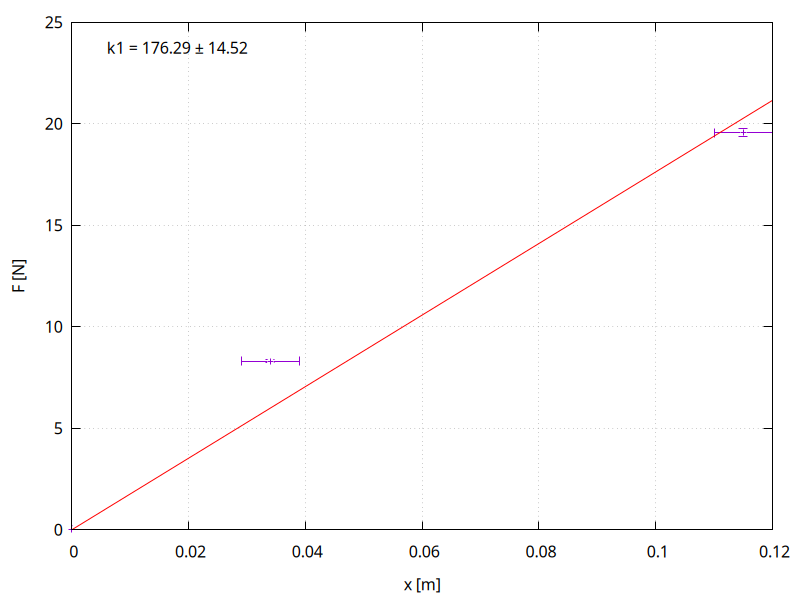
\includegraphics[width=0.5\textwidth]{vzmet1}
        \caption{Graf2}
        \label{fig:1}
    \end{figure}
    \begin{figure}[H]
        \centering
        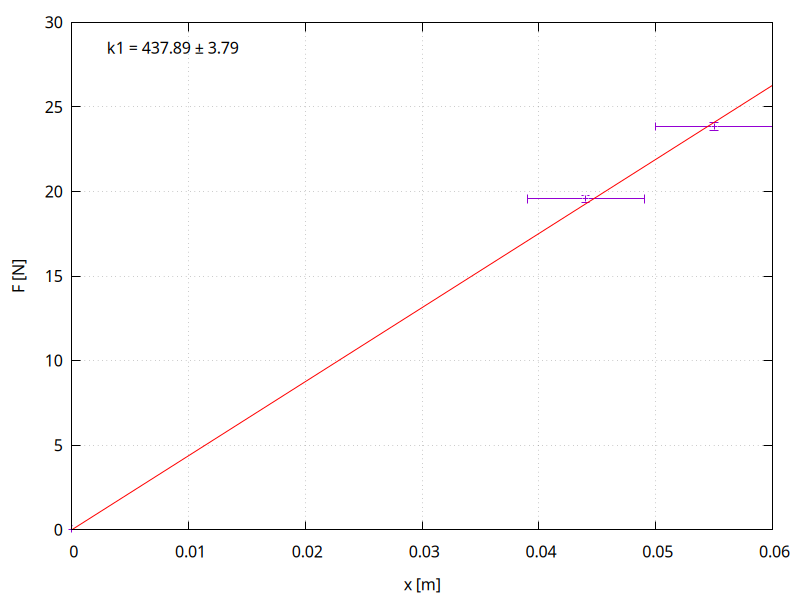
\includegraphics[width=0.5\textwidth]{vzmet2}
        \caption{Graf2}
        \label{fig:2}
    \end{figure}
    \begin{figure}[H]
        \centering
        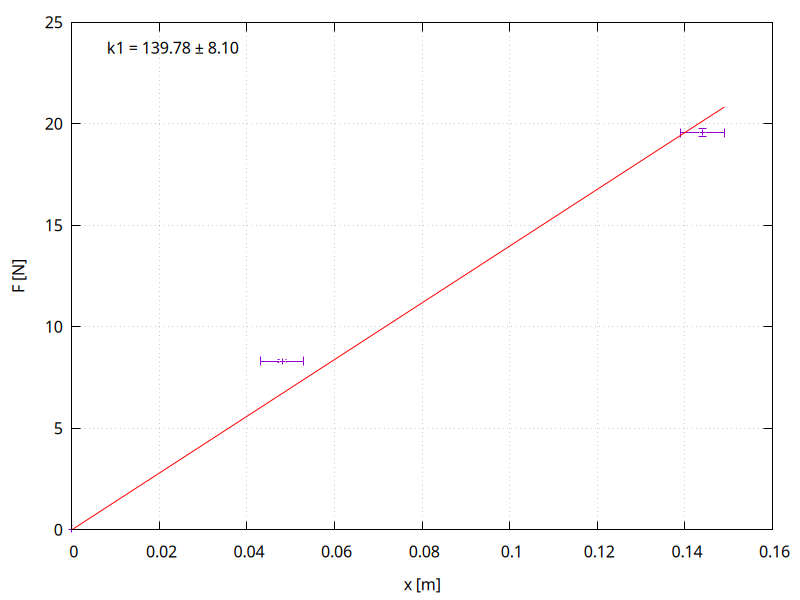
\includegraphics[width=0.5\textwidth]{vzmet3}
        \caption{Graf3}
        \label{fig:3}
    \end{figure}
    \begin{figure}[H]
        \centering
        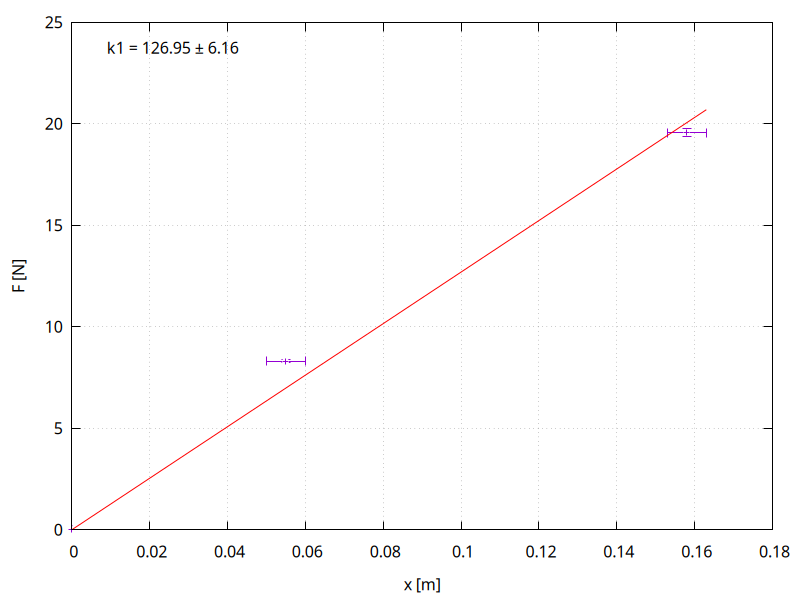
\includegraphics[width=0.5\textwidth]{vzmet4}
        \caption{Graf4}
        \label{fig:4}
    \end{figure}
    \begin{figure}[H]
        \centering
        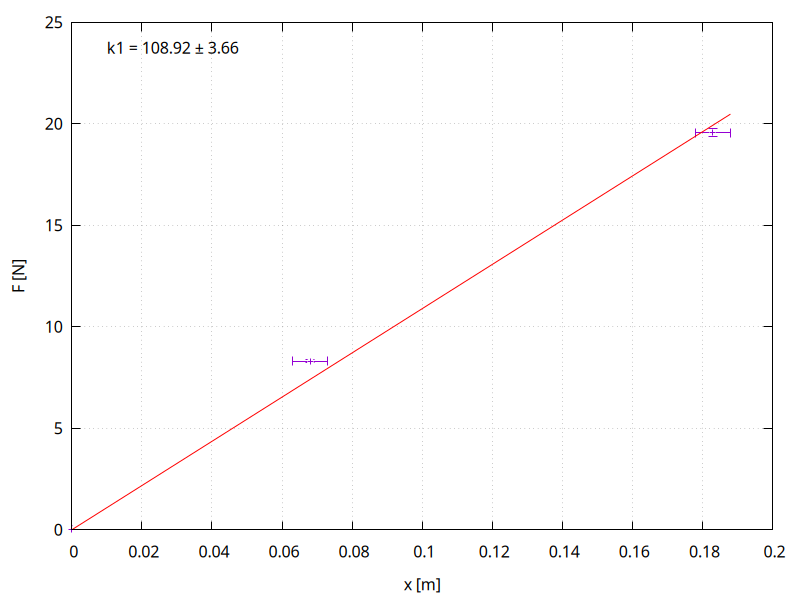
\includegraphics[width=0.5\textwidth]{vzmet5}
        \caption{Graf5}
        \label{fig:5}
    \end{figure}
    \begin{figure}[H]
        \centering
        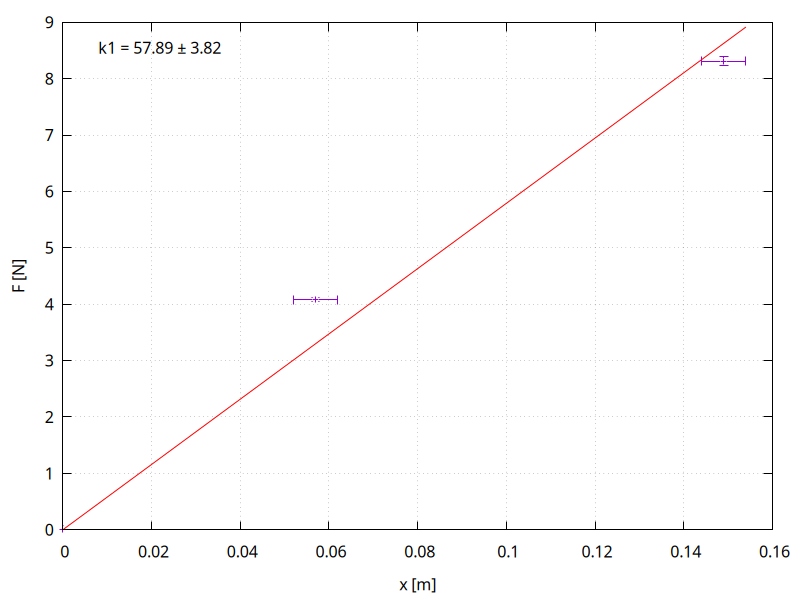
\includegraphics[width=0.5\textwidth]{vzmet6}
        \caption{Graf6}
        \label{fig:6}
    \end{figure}
    \begin{figure}[H]
        \centering
        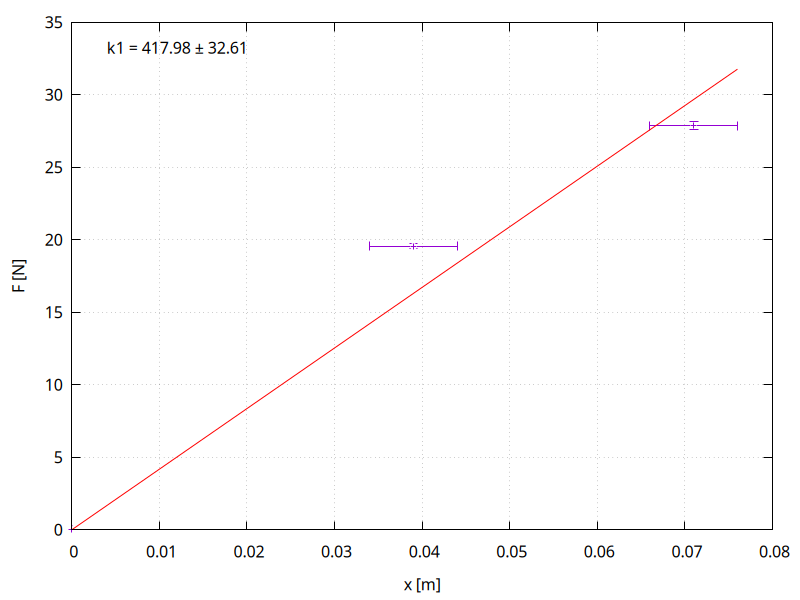
\includegraphics[width=0.5\textwidth]{vzmet7}
        \caption{Graf7}
        \label{fig:7}
    \end{figure}

    V sledeči tabeli so koeficienti vzmeti in tudi njihove geometrijske lastnosti:


    % ne dotikaj se te tabele
\begin{table}[H]
        \centering
        \begin{tabular}{rrllrlrr}
            \textbf{} & \textbf{k} & \textbf{} & \textbf{} & \textbf{D} & \textbf{} & \textbf{N} & \textbf{d} \\
            1 & 180 &
 &
 & 0.0263 &
 & 78 & 0.00202 \\
            2 & 438 &
 &
 & 0.0198 &
 & 78 & 0.00202 \\
            3 & 140 &
 &
 & 0.0263 &
 & 98 & 0.00202 \\
            4 & 127 &
 &
 & 0.0291 &
 & 78 & 0.00202 \\
            5 & 109 &
 &
 & 0.0263 &
 & 117 & 0.00202 \\
            6 & 58 &
 &
 & 0.038 &
 & 78 & 0.00202 \\
            7 & 420 &
 &
 & 0.0291 &
 & 78 & 0.00252 \\
        \end{tabular}
        \caption{}
        \label{tab:}
    \end{table}

    \section{Računi}
    Vzmeti, ki imajo isti N,d  ampak različne D (premer celotnega zavoja) so: 1,2,4,6
    Ker imamo to enačbo:
    \[
        \ln k = \ln (\frac{G d^4}{8n}) -\alpha \ln D
    \]
    Jo lahko lineariziramo...
    Spodnji graf vsebije linearizacijo:
    \begin{figure}[H]
        \centering
        
\includegraphics[width=0.9\textwidth]{graf1}
        \caption{Graf1}
        \label{fig:10}
    \end{figure}
    Kot vidimo se podatki strinjajo z enačbo.
    Prosti člen pa je $\alpha = (3.11 \pm 0.03)$
    Tako lahko določimo strižnostni modul žice (prosti člen $y_0 = -2.66$):
    \[
        e^{y_0} *\frac{8n}{d^4} = G
    \]
    Torej za:
    \[
        G_{1,2,4,6} = 2.6 * 10^{12} N/m^2
    \]

    2. del:
    Vzmeti katere se razlikujejo v premeru žice d sta vzmet 4 in 7.
    Lineariziramo z enačbo:
    \[
        \ln(k) = \ln(\frac{G}{8 n D^3}) + \beta \ln(d)
    \]
    Spodnji graf vsebije linearizacijo:
    \begin{figure}[H]
        \centering
        
\includegraphics[width=0.9\textwidth]{graf2}
        \caption{Graf1}
        \label{fig:11}
    \end{figure}
    Tako je :
    \[
        \ln(\frac{G}{8 n D^3}) = y_0
    \]
    Torej:
    \[
        e^{y_0} *8 n D^3 = G
    \]
    Vsatvimo, dobimo:
    \[
        G = 2.6 * 10^{12} N/m^2
    \]

    Dobimo isti rezultat, torej so vzmeti narejene iz istega materijala in teorija štima!

\end{document}